\documentclass[]{article}
\usepackage{lmodern}
\usepackage{amssymb,amsmath}
\usepackage{ifxetex,ifluatex}
\usepackage{fixltx2e} % provides \textsubscript
\ifnum 0\ifxetex 1\fi\ifluatex 1\fi=0 % if pdftex
  \usepackage[T1]{fontenc}
  \usepackage[utf8]{inputenc}
\else % if luatex or xelatex
  \ifxetex
    \usepackage{mathspec}
  \else
    \usepackage{fontspec}
  \fi
  \defaultfontfeatures{Ligatures=TeX,Scale=MatchLowercase}
\fi
% use upquote if available, for straight quotes in verbatim environments
\IfFileExists{upquote.sty}{\usepackage{upquote}}{}
% use microtype if available
\IfFileExists{microtype.sty}{%
\usepackage{microtype}
\UseMicrotypeSet[protrusion]{basicmath} % disable protrusion for tt fonts
}{}
\usepackage[margin=1in]{geometry}
\usepackage{hyperref}
\hypersetup{unicode=true,
            pdftitle={Week 2 Assignment},
            pdfauthor={Adam Douglas},
            pdfborder={0 0 0},
            breaklinks=true}
\urlstyle{same}  % don't use monospace font for urls
\usepackage{color}
\usepackage{fancyvrb}
\newcommand{\VerbBar}{|}
\newcommand{\VERB}{\Verb[commandchars=\\\{\}]}
\DefineVerbatimEnvironment{Highlighting}{Verbatim}{commandchars=\\\{\}}
% Add ',fontsize=\small' for more characters per line
\usepackage{framed}
\definecolor{shadecolor}{RGB}{248,248,248}
\newenvironment{Shaded}{\begin{snugshade}}{\end{snugshade}}
\newcommand{\KeywordTok}[1]{\textcolor[rgb]{0.13,0.29,0.53}{\textbf{#1}}}
\newcommand{\DataTypeTok}[1]{\textcolor[rgb]{0.13,0.29,0.53}{#1}}
\newcommand{\DecValTok}[1]{\textcolor[rgb]{0.00,0.00,0.81}{#1}}
\newcommand{\BaseNTok}[1]{\textcolor[rgb]{0.00,0.00,0.81}{#1}}
\newcommand{\FloatTok}[1]{\textcolor[rgb]{0.00,0.00,0.81}{#1}}
\newcommand{\ConstantTok}[1]{\textcolor[rgb]{0.00,0.00,0.00}{#1}}
\newcommand{\CharTok}[1]{\textcolor[rgb]{0.31,0.60,0.02}{#1}}
\newcommand{\SpecialCharTok}[1]{\textcolor[rgb]{0.00,0.00,0.00}{#1}}
\newcommand{\StringTok}[1]{\textcolor[rgb]{0.31,0.60,0.02}{#1}}
\newcommand{\VerbatimStringTok}[1]{\textcolor[rgb]{0.31,0.60,0.02}{#1}}
\newcommand{\SpecialStringTok}[1]{\textcolor[rgb]{0.31,0.60,0.02}{#1}}
\newcommand{\ImportTok}[1]{#1}
\newcommand{\CommentTok}[1]{\textcolor[rgb]{0.56,0.35,0.01}{\textit{#1}}}
\newcommand{\DocumentationTok}[1]{\textcolor[rgb]{0.56,0.35,0.01}{\textbf{\textit{#1}}}}
\newcommand{\AnnotationTok}[1]{\textcolor[rgb]{0.56,0.35,0.01}{\textbf{\textit{#1}}}}
\newcommand{\CommentVarTok}[1]{\textcolor[rgb]{0.56,0.35,0.01}{\textbf{\textit{#1}}}}
\newcommand{\OtherTok}[1]{\textcolor[rgb]{0.56,0.35,0.01}{#1}}
\newcommand{\FunctionTok}[1]{\textcolor[rgb]{0.00,0.00,0.00}{#1}}
\newcommand{\VariableTok}[1]{\textcolor[rgb]{0.00,0.00,0.00}{#1}}
\newcommand{\ControlFlowTok}[1]{\textcolor[rgb]{0.13,0.29,0.53}{\textbf{#1}}}
\newcommand{\OperatorTok}[1]{\textcolor[rgb]{0.81,0.36,0.00}{\textbf{#1}}}
\newcommand{\BuiltInTok}[1]{#1}
\newcommand{\ExtensionTok}[1]{#1}
\newcommand{\PreprocessorTok}[1]{\textcolor[rgb]{0.56,0.35,0.01}{\textit{#1}}}
\newcommand{\AttributeTok}[1]{\textcolor[rgb]{0.77,0.63,0.00}{#1}}
\newcommand{\RegionMarkerTok}[1]{#1}
\newcommand{\InformationTok}[1]{\textcolor[rgb]{0.56,0.35,0.01}{\textbf{\textit{#1}}}}
\newcommand{\WarningTok}[1]{\textcolor[rgb]{0.56,0.35,0.01}{\textbf{\textit{#1}}}}
\newcommand{\AlertTok}[1]{\textcolor[rgb]{0.94,0.16,0.16}{#1}}
\newcommand{\ErrorTok}[1]{\textcolor[rgb]{0.64,0.00,0.00}{\textbf{#1}}}
\newcommand{\NormalTok}[1]{#1}
\usepackage{graphicx,grffile}
\makeatletter
\def\maxwidth{\ifdim\Gin@nat@width>\linewidth\linewidth\else\Gin@nat@width\fi}
\def\maxheight{\ifdim\Gin@nat@height>\textheight\textheight\else\Gin@nat@height\fi}
\makeatother
% Scale images if necessary, so that they will not overflow the page
% margins by default, and it is still possible to overwrite the defaults
% using explicit options in \includegraphics[width, height, ...]{}
\setkeys{Gin}{width=\maxwidth,height=\maxheight,keepaspectratio}
\IfFileExists{parskip.sty}{%
\usepackage{parskip}
}{% else
\setlength{\parindent}{0pt}
\setlength{\parskip}{6pt plus 2pt minus 1pt}
}
\setlength{\emergencystretch}{3em}  % prevent overfull lines
\providecommand{\tightlist}{%
  \setlength{\itemsep}{0pt}\setlength{\parskip}{0pt}}
\setcounter{secnumdepth}{0}
% Redefines (sub)paragraphs to behave more like sections
\ifx\paragraph\undefined\else
\let\oldparagraph\paragraph
\renewcommand{\paragraph}[1]{\oldparagraph{#1}\mbox{}}
\fi
\ifx\subparagraph\undefined\else
\let\oldsubparagraph\subparagraph
\renewcommand{\subparagraph}[1]{\oldsubparagraph{#1}\mbox{}}
\fi

%%% Use protect on footnotes to avoid problems with footnotes in titles
\let\rmarkdownfootnote\footnote%
\def\footnote{\protect\rmarkdownfootnote}

%%% Change title format to be more compact
\usepackage{titling}

% Create subtitle command for use in maketitle
\newcommand{\subtitle}[1]{
  \posttitle{
    \begin{center}\large#1\end{center}
    }
}

\setlength{\droptitle}{-2em}

  \title{Week 2 Assignment}
    \pretitle{\vspace{\droptitle}\centering\huge}
  \posttitle{\par}
    \author{Adam Douglas}
    \preauthor{\centering\large\emph}
  \postauthor{\par}
      \predate{\centering\large\emph}
  \postdate{\par}
    \date{9/7/2018}


\begin{document}
\maketitle

\subsection{The Database}\label{the-database}

We begin by creating a database to store our movies, raters, and ratings
in. For this exercise, I have chosen PostgreSQL. Not only is it a
popular open source choice and a robust DBMS, but it is also one of the
DBMS I have not used yet so I wanted to give it a try.

\subsubsection{The Structure}\label{the-structure}

The structure of the database will be simple enough. One table with
movies in it, one with people who see one or more of the movies, and an
associative table with each person's ratings. Below is a basic ER
diagram outlining the general structure:

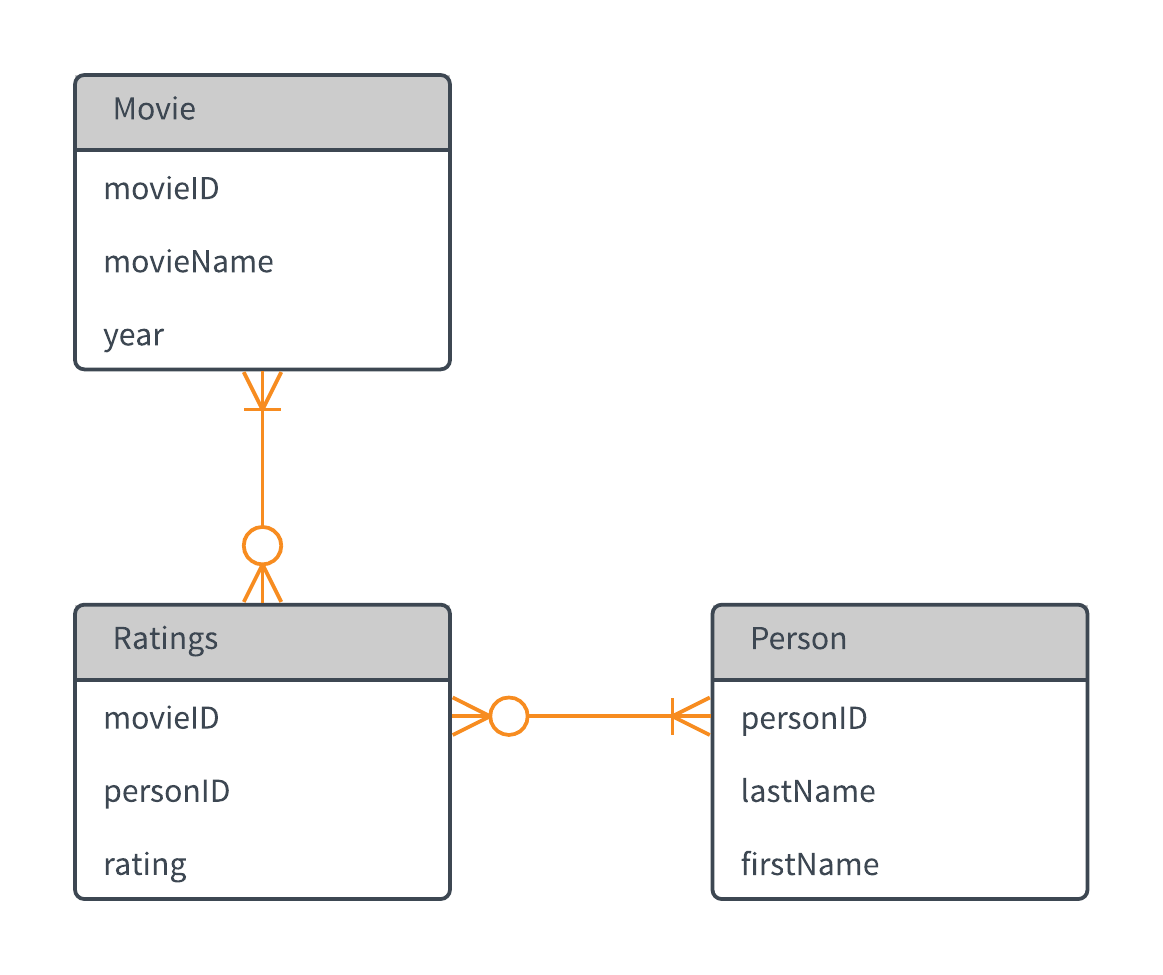
\includegraphics{https://raw.githubusercontent.com/lysanthus/Data607/master/Week\%202/db.png}

\subsubsection{The Code}\label{the-code}

Once we have our structure set, we begin creating the tables themselves.
The code used to create the tables in the PostgreSQL database system and
load the data into them is included in a separate file called
\texttt{Assignment\ 2.sql}. To give an idea of what the structure looks
like from a code perspective, below are the table creation statements
used:

\begin{quote}
CREATE TABLE public.movies ( ``movieID'' integer NOT NULL, ``movieName''
character varying(200), year integer, CONSTRAINT movies\_pkey PRIMARY
KEY (``movieID''))
\end{quote}

\begin{quote}
CREATE TABLE public.person ( ``personID'' integer NOT NULL, ``lastName''
character varying(20), ``firstName'' character varying(40), CONSTRAINT
person\_pkey PRIMARY KEY (``personID'') )
\end{quote}

\begin{quote}
CREATE TABLE public.ratings ( ``movieID'' integer, ``personID'' integer,
rating integer, PRIMARY KEY (``movieID'', ``personID''), CONSTRAINT
fk\_movie FOREIGN KEY (``movieID'') REFERENCES public.movies
(``movieID''), CONSTRAINT fk\_person FOREIGN KEY (``personID'')
REFERENCES public.person (``personID''), CONSTRAINT ck\_rating CHECK
(rating \textgreater{}= 1 AND rating \textless{}= 5) )
\end{quote}

Note that the ratings table has a few constraints on it. First it uses
foreign keys to ensure that any \texttt{movieID} or \texttt{personID}
put into it has a match in their respective tables. Also, we use a check
constraint to ensure that ratings are from 1 - 5 stars.

\begin{center}\rule{0.5\linewidth}{\linethickness}\end{center}

\subsection{The Data}\label{the-data}

Now that we have the data loaded into our database, we will need to
query it to do any kind of analysis. We begin by loading the package
we'll use to connect to the PostgreSQL database and setting up some
basic variables with information about the database itself (such as
user, password, what port it is running on, etc.):

\begin{Shaded}
\begin{Highlighting}[]
\CommentTok{# Load the package to connect}
\KeywordTok{library}\NormalTok{(RPostgreSQL)}

\CommentTok{# Variables to create the connection}
\NormalTok{host <-}\StringTok{ "localhost"}
\NormalTok{usr <-}\StringTok{ "postgres"}
\NormalTok{pass <-}\StringTok{ }\NormalTok{params}\OperatorTok{$}\NormalTok{password}
\NormalTok{port <-}\StringTok{ }\DecValTok{5432}
\NormalTok{database <-}\StringTok{ "movies"}
\end{Highlighting}
\end{Shaded}

Now we create the actual driver and connection:

\begin{Shaded}
\begin{Highlighting}[]
\CommentTok{# Creates the actual connection object}
\NormalTok{conn <-}\StringTok{ }\KeywordTok{dbConnect}\NormalTok{(RPostgreSQL}\OperatorTok{::}\KeywordTok{PostgreSQL}\NormalTok{(),}\DataTypeTok{host =}\NormalTok{ host, }\DataTypeTok{dbname =}\NormalTok{ database, }\DataTypeTok{user =}\NormalTok{ usr, }\DataTypeTok{password =}\NormalTok{ pass)}
\end{Highlighting}
\end{Shaded}

Now that we have the connection object, let's test to make sure it
works:

\begin{Shaded}
\begin{Highlighting}[]
\CommentTok{# A test SQL query}
\NormalTok{testSQL <-}\StringTok{ }\KeywordTok{dbSendQuery}\NormalTok{(conn, }\StringTok{"select count(*) from public.movies"}\NormalTok{)}

\CommentTok{# Retreive the results}
\NormalTok{test <-}\StringTok{ }\KeywordTok{dbFetch}\NormalTok{(testSQL)}
\end{Highlighting}
\end{Shaded}

We see from the results that we have 6 records in the \texttt{movies}
table, which is what we expect.

Now, we will aquire the data. Rather than writing a single query
combining the tables, I'm going to pull each one into its own object and
work with them within R. I am doing this for two reasons:

\begin{enumerate}
\def\labelenumi{\arabic{enumi}.}
\item
  I am not sure yet what sort of analysis I want to perform on the data.
  If I have the data as a result of a SQL statement, I need to decide
  what I want when I execute that SQL. This way I can adapt as I go by
  filtering the data in its raw form within R.
\item
  It gives me an opportunity to work with \texttt{dplyr} and other tools
  to format and tidy data.
\end{enumerate}

\begin{Shaded}
\begin{Highlighting}[]
\CommentTok{# Get the movies}
\NormalTok{movieSQL <-}\StringTok{ }\KeywordTok{dbSendQuery}\NormalTok{(conn, }\StringTok{"select * from public.movies"}\NormalTok{)}
\NormalTok{movies <-}\StringTok{ }\KeywordTok{dbFetch}\NormalTok{(movieSQL)}
\CommentTok{# Get the people}
\NormalTok{personSQL <-}\StringTok{ }\KeywordTok{dbSendQuery}\NormalTok{(conn, }\StringTok{"select * from public.person"}\NormalTok{)}
\NormalTok{person <-}\StringTok{ }\KeywordTok{dbFetch}\NormalTok{(personSQL)}
\CommentTok{# Get the ratings}
\NormalTok{ratingsSQL <-}\StringTok{ }\KeywordTok{dbSendQuery}\NormalTok{(conn, }\StringTok{"select * from public.ratings"}\NormalTok{)}
\NormalTok{ratings <-}\StringTok{ }\KeywordTok{dbFetch}\NormalTok{(ratingsSQL)}
\end{Highlighting}
\end{Shaded}

Now that we have our data, we can close the database connection:

\begin{Shaded}
\begin{Highlighting}[]
\KeywordTok{dbDisconnect}\NormalTok{(conn)}
\end{Highlighting}
\end{Shaded}

\begin{center}\rule{0.5\linewidth}{\linethickness}\end{center}

\subsection{The Analysis}\label{the-analysis}

First let's look at the data we've gathered:

\begin{Shaded}
\begin{Highlighting}[]
\KeywordTok{str}\NormalTok{(movies)}
\end{Highlighting}
\end{Shaded}

\begin{verbatim}
## 'data.frame':    6 obs. of  3 variables:
##  $ movieID  : int  1 2 3 4 5 6
##  $ movieName: chr  "Avengers: Infinity War" "BlacKkKlansman" "Crazy Rich Asians" "Won't You Be My Neighbor?" ...
##  $ year     : int  2018 2018 2018 2018 2018 2017
\end{verbatim}

\begin{Shaded}
\begin{Highlighting}[]
\KeywordTok{str}\NormalTok{(person)}
\end{Highlighting}
\end{Shaded}

\begin{verbatim}
## 'data.frame':    5 obs. of  3 variables:
##  $ personID : int  1 2 3 4 5
##  $ lastName : chr  "Douglas" "Douglas" "Douglas" "Douglas" ...
##  $ firstName: chr  "Adam" "April" "Amber" "Tyler" ...
\end{verbatim}

\begin{Shaded}
\begin{Highlighting}[]
\KeywordTok{str}\NormalTok{(ratings)}
\end{Highlighting}
\end{Shaded}

\begin{verbatim}
## 'data.frame':    21 obs. of  3 variables:
##  $ movieID : int  1 1 1 2 2 2 3 3 3 4 ...
##  $ personID: int  1 4 5 1 2 3 2 3 5 1 ...
##  $ rating  : int  5 4 5 4 3 4 4 5 5 5 ...
\end{verbatim}

We have both int variables and character variables, which is what we
expected from the database.

First, let's look at who is doing how many ratings. Before we can answer
this, and other, questions, we need to combine these datasets into a
single tidy dataset. We will do this by using joining functions courtesy
of the \texttt{dplyr} package, which is part of the Tidyverse set of
packages; the syntax is similar to SQL.

Let's look at everyone's ratings, regardless of the movie:

\begin{Shaded}
\begin{Highlighting}[]
\CommentTok{# We combine the datasets and select only the fields we want}
\NormalTok{ratingsByPerson <-}\StringTok{ }\NormalTok{movies }\OperatorTok\StringTok{ }\KeywordTok{left_join}\NormalTok{(ratings, }\DataTypeTok{by=}\StringTok{"movieID"}\NormalTok{) }\OperatorTok\StringTok{ }\KeywordTok{inner_join}\NormalTok{(person, }\DataTypeTok{by=}\StringTok{"personID"}\NormalTok{) }\OperatorTok\StringTok{ }\KeywordTok{select}\NormalTok{(firstName, rating)}

\KeywordTok{glimpse}\NormalTok{(ratingsByPerson)}
\end{Highlighting}
\end{Shaded}

\begin{verbatim}
## Observations: 21
## Variables: 2
## $ firstName <chr> "Adam", "Tyler", "Brianna", "Adam", "April", "Amber"...
## $ rating    <int> 5, 4, 5, 4, 3, 4, 4, 5, 5, 5, 5, 4, 3, 4, 4, 3, 2, 4...
\end{verbatim}

\begin{Shaded}
\begin{Highlighting}[]
\KeywordTok{ggplot}\NormalTok{(ratingsByPerson, }\KeywordTok{aes}\NormalTok{(rating, }\DataTypeTok{fill=}\NormalTok{firstName)) }\OperatorTok{+}\StringTok{ }\KeywordTok{geom_bar}\NormalTok{() }\OperatorTok{+}\StringTok{ }\KeywordTok{scale_y_continuous}\NormalTok{(}\DataTypeTok{breaks=}\KeywordTok{seq}\NormalTok{(}\DecValTok{0}\NormalTok{,}\DecValTok{10}\NormalTok{,}\DecValTok{2}\NormalTok{)) }\OperatorTok{+}\StringTok{ }\KeywordTok{labs}\NormalTok{(}\DataTypeTok{title=}\StringTok{"Ratings by Person"}\NormalTok{, }\DataTypeTok{x=}\StringTok{"Rating"}\NormalTok{, }\DataTypeTok{y=}\StringTok{"Count"}\NormalTok{, }\DataTypeTok{fill=}\StringTok{"Person"}\NormalTok{)}
\end{Highlighting}
\end{Shaded}

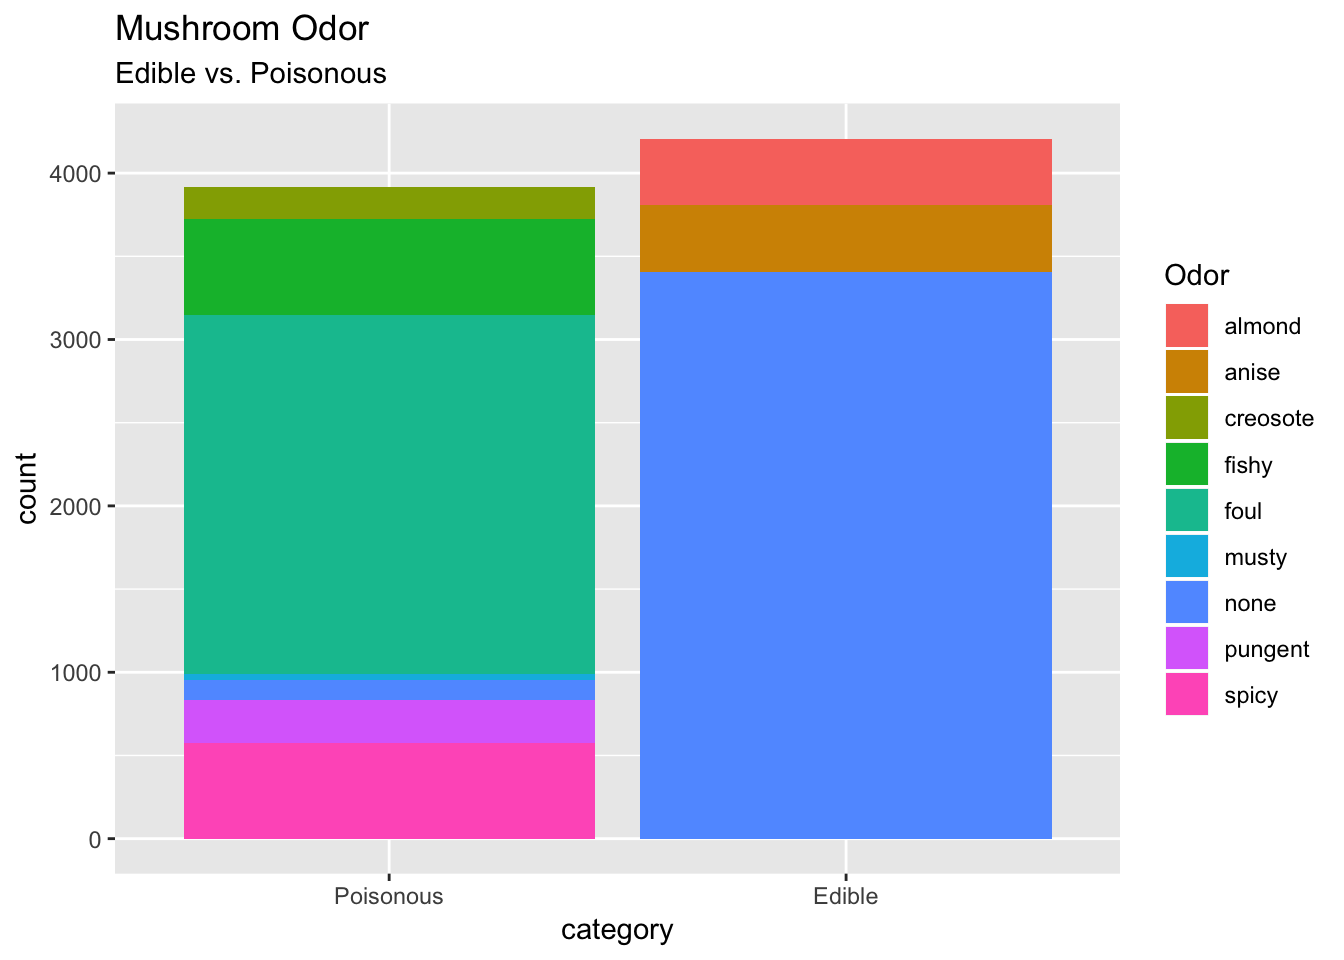
\includegraphics{Data_607_-_Week_2_Assignment_files/figure-latex/unnamed-chunk-9-1.pdf}

Looking at the distribution of ratings, it appears that I (Adam) tend to
rate high (only 4's or 5's) and my wife (April) tends to rate more
evenly across the 3-4 range. Perhaps I need to choose the movies less
often.

Now let's look at how individual movies fared overall:

\begin{Shaded}
\begin{Highlighting}[]
\CommentTok{# Like before, we combine the datasets and select only the fields we want}
\NormalTok{ratingsByMovie <-}\StringTok{ }\NormalTok{movies }\OperatorTok\StringTok{ }\KeywordTok{left_join}\NormalTok{(ratings, }\DataTypeTok{by=}\StringTok{"movieID"}\NormalTok{) }\OperatorTok\StringTok{ }\KeywordTok{select}\NormalTok{(movieName, rating)}

\KeywordTok{glimpse}\NormalTok{(ratingsByMovie)}
\end{Highlighting}
\end{Shaded}

\begin{verbatim}
## Observations: 21
## Variables: 2
## $ movieName <chr> "Avengers: Infinity War", "Avengers: Infinity War", ...
## $ rating    <int> 5, 4, 5, 4, 3, 4, 4, 5, 5, 5, 5, 4, 3, 4, 4, 3, 2, 4...
\end{verbatim}

Let's get a sense of how the movies fared in terms of typical ratings:

\begin{Shaded}
\begin{Highlighting}[]
\NormalTok{ratingsByMovie }\OperatorTok\StringTok{ }\KeywordTok{group_by}\NormalTok{(movieName) }\OperatorTok\StringTok{ }\KeywordTok{summarize}\NormalTok{(}\DataTypeTok{AvgRating =} \KeywordTok{mean}\NormalTok{(rating), }\DataTypeTok{NumRatings =} \KeywordTok{n}\NormalTok{()) }\OperatorTok\StringTok{ }\KeywordTok{arrange}\NormalTok{(}\KeywordTok{desc}\NormalTok{(AvgRating),movieName)}
\end{Highlighting}
\end{Shaded}

\begin{verbatim}
## # A tibble: 6 x 3
##   movieName                                  AvgRating NumRatings
##   <chr>                                          <dbl>      <int>
## 1 Avengers: Infinity War                          4.67          3
## 2 Crazy Rich Asians                               4.67          3
## 3 Three BIillboards Outside Ebbing, Missouri      4.67          3
## 4 Won't You Be My Neighbor?                       4.2           5
## 5 BlacKkKlansman                                  3.67          3
## 6 A Quiet Place                                   3.25          4
\end{verbatim}

``Avengers: Infinity War'', ``Crazy Rich Asians'', and ``Three
Billboards Outside Ebbing, Missouri'' are the most popular when one
looks at mean ratings. The Mr.~Roger's documentary ``Won't You Be My
Neighbor'' had the most appeal amongst the family, as it had the largest
number of ratings overall (and got a 4.2 mean rating!).

Finally, let's look at how each person rated each individual movie:

\begin{Shaded}
\begin{Highlighting}[]
\CommentTok{# Once again, we select just what we need}
\NormalTok{ratingsByMovieByPerson <-}\StringTok{ }\NormalTok{movies }\OperatorTok\StringTok{ }\KeywordTok{left_join}\NormalTok{(ratings, }\DataTypeTok{by=}\StringTok{"movieID"}\NormalTok{) }\OperatorTok\StringTok{ }\KeywordTok{inner_join}\NormalTok{(person, }\DataTypeTok{by=}\StringTok{"personID"}\NormalTok{) }\OperatorTok\StringTok{ }\KeywordTok{select}\NormalTok{(movieName, firstName, rating)}

\KeywordTok{glimpse}\NormalTok{(ratingsByMovieByPerson)}
\end{Highlighting}
\end{Shaded}

\begin{verbatim}
## Observations: 21
## Variables: 3
## $ movieName <chr> "Avengers: Infinity War", "Avengers: Infinity War", ...
## $ firstName <chr> "Adam", "Tyler", "Brianna", "Adam", "April", "Amber"...
## $ rating    <int> 5, 4, 5, 4, 3, 4, 4, 5, 5, 5, 5, 4, 3, 4, 4, 3, 2, 4...
\end{verbatim}

Let's take a numerical look at ``Avengers: Infinity War'', as an
example:

\begin{Shaded}
\begin{Highlighting}[]
\NormalTok{ratingsByMovieByPerson }\OperatorTok\StringTok{ }\KeywordTok{filter}\NormalTok{(movieName }\OperatorTok{==}\StringTok{ "Avengers: Infinity War"}\NormalTok{)}
\end{Highlighting}
\end{Shaded}

\begin{verbatim}
##                movieName firstName rating
## 1 Avengers: Infinity War      Adam      5
## 2 Avengers: Infinity War     Tyler      4
## 3 Avengers: Infinity War   Brianna      5
\end{verbatim}

Three people rated the movie, and overall it was rated very well.

However, rather than look at each one individually, we can visualize the
ratings by person and movie in one graphic:

\begin{Shaded}
\begin{Highlighting}[]
\KeywordTok{ggplot}\NormalTok{(ratingsByMovieByPerson, }\KeywordTok{aes}\NormalTok{(firstName, movieName)) }\OperatorTok{+}\StringTok{ }\KeywordTok{geom_tile}\NormalTok{(}\KeywordTok{aes}\NormalTok{(}\DataTypeTok{fill=}\KeywordTok{as.factor}\NormalTok{(rating))) }\OperatorTok{+}\StringTok{ }\KeywordTok{scale_fill_brewer}\NormalTok{(}\DataTypeTok{name=}\StringTok{"Rating"}\NormalTok{,}\DataTypeTok{palette=}\StringTok{"RdYlGn"}\NormalTok{) }\OperatorTok{+}\StringTok{ }\KeywordTok{geom_text}\NormalTok{(}\KeywordTok{aes}\NormalTok{(}\DataTypeTok{label=}\NormalTok{rating)) }\OperatorTok{+}\StringTok{ }\KeywordTok{guides}\NormalTok{(}\DataTypeTok{fill=}\OtherTok{FALSE}\NormalTok{) }\OperatorTok{+}\StringTok{ }\KeywordTok{labs}\NormalTok{(}\DataTypeTok{title=}\StringTok{"Movie Ratings by Person"}\NormalTok{, }\DataTypeTok{x=}\StringTok{""}\NormalTok{, }\DataTypeTok{y=}\StringTok{""}\NormalTok{)}
\end{Highlighting}
\end{Shaded}

\includegraphics{Data_607_-_Week_2_Assignment_files/figure-latex/unnamed-chunk-14-1.pdf}

\begin{center}\rule{0.5\linewidth}{\linethickness}\end{center}


\end{document}
